\documentclass[11pt]{article}
\usepackage{hw-solutions-common}
\usepackage{tikz}
\usetikzlibrary{arrows.meta,decorations.markings}

\begin{document}

\hwsolhead{Written HW 7}{Problem statements from Knight, \emph{Physics for Scientists and
Engineers} (5th ed., Global Edition), Chapter 29. $\mu_0 = 4\pi\times10^{-7}\text{
T}\cdot\text{m/A}$ throughout.}

%============================================================
\problem{29.11}{2}{Exercise 29.10 establishes a long straight wire carrying a current of
200 A (that value is carried over here; 29.10 itself isn't assigned). At what distance
from the wire does the magnetic field strength equal 2.2 mT?}

\model{A long straight wire's field circles the wire in loops of constant magnitude at
fixed radius, $B=\mu_0 I/(2\pi r)$, with direction set by the right-hand rule. Here we
know $B$ and solve for the radius $r$ instead of the other way around.}

\visualize{
\begin{center}
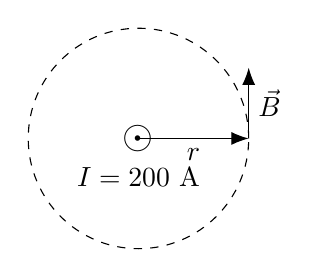
\begin{tikzpicture}[scale=1]
\node at (0,0) {\Large $\odot$};
\node[below] at (0,-0.25) {$I=200$ A};
\draw[dashed] (0,0) circle (1.4);
\draw[-{Latex[length=2.2mm]}] (0,0) -- (1.4,0);
\node[below] at (0.7,0) {$r$};
\draw[-{Latex[length=2.2mm]}] (1.4,0) -- (1.4,0.9);
\node[right] at (1.4,0.45) {$\vec B$};
\end{tikzpicture}
\end{center}
The field lines are circles centered on the wire; $\vec B$ is everywhere tangent to
these circles. We just need the one circle whose field strength is 2.2 mT.}

\solve{
\[
B=\frac{\mu_0 I}{2\pi r} \;\Rightarrow\; r=\frac{\mu_0 I}{2\pi B}
=\frac{(4\pi\times10^{-7}\text{ T}\cdot\text{m/A})(200\text{ A})}{2\pi(2.2\times10^{-3}\text{
T})} = \boxed{1.8\text{ cm}}.
\]}

\review{A field of a couple mT this close to a wire carrying hundreds of amps is
reasonable --- for comparison, Earth's field ($\sim$0.05 mT) is roughly 40 times weaker,
and we're well inside where a 200 A wire dominates.}

%============================================================
\problem{29.15}{2}{Two concentric circular loops of radii 1.0 cm and 2.0 cm carry equal
currents $I$ in opposite directions. The magnetic field at their common center has
strength 350 $\mu$T. What is $I$?}

\model{Each loop produces a field at its own center of $B=\mu_0 I/(2R)$, directed along
the axis by the right-hand rule. Because the two currents circulate in opposite senses,
their center-fields point in opposite directions and partially cancel.}

\visualize{
\begin{center}
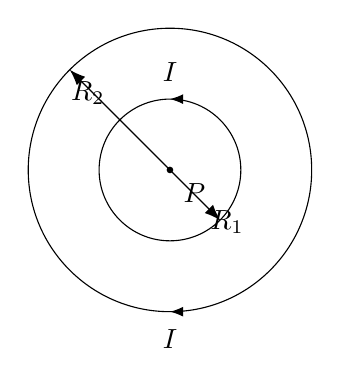
\begin{tikzpicture}[scale=1]
\draw[postaction={decorate},decoration={markings,mark=at position 0.25 with {\arrow{Latex}}}]
  (0,0) circle (0.9);
\draw[postaction={decorate},decoration={markings,mark=at position 0.25 with {\arrow{Latex}}}]
  (1.8,0) arc (0:-360:1.8);
\fill (0,0) circle (1.2pt);
\node[below right] at (0.05,-0.05) {$P$};
\draw[-{Latex[length=2mm]}] (0,0) -- (-45:0.9);
\node[below right] at (-45:0.55) {$R_1$};
\draw[-{Latex[length=2mm]}] (0,0) -- (135:1.8);
\node[above left] at (135:1.0) {$R_2$};
\node[above] at (0,1.0) {$I$};
\node[below] at (0,-1.9) {$I$};
\end{tikzpicture}
\end{center}
With $R_1=1.0$ cm (inner, drawn circulating counterclockwise) and $R_2=2.0$ cm (outer,
circulating clockwise), the net field at $P$ is the \emph{difference} of the two
loops' individual fields, since they point opposite ways along the common axis.}

\solve{
\[
B = \frac{\mu_0 I}{2}\left(\frac{1}{R_1}-\frac{1}{R_2}\right)
\;\Rightarrow\;
I = \frac{2B}{\mu_0\left(\dfrac{1}{R_1}-\dfrac{1}{R_2}\right)}
\]
\[
\frac{1}{R_1}-\frac{1}{R_2} = \frac{1}{0.010\text{ m}}-\frac{1}{0.020\text{ m}} = 100 -
50 = 50\text{ m}^{-1}
\]
\[
I = \frac{2(350\times10^{-6}\text{ T})}{(4\pi\times10^{-7}\text{ T}\cdot\text{m/A})(50\text{
m}^{-1})} = \boxed{11\text{ A}}.
\]}

\review{Because the smaller loop is twice as effective per amp ($1/R_1=2/R_2$), the
cancellation only removes half of the inner loop's contribution --- the combination
still behaves like a single loop of radius 2 cm, which is why a modest 11 A gives a
healthy 350 $\mu$T despite the two fields opposing each other.}

%============================================================
\problem{29.16}{2}{A 4.0-mm-diameter circular loop of wire carries a current of 150 A.
(a) What is the loop's magnetic dipole moment? (b) What is the on-axis magnetic field
strength at a point 10.0 cm from the loop's center?}

\model{A current loop's dipole moment is $m=IA$, directed along the axis by the
right-hand rule. Far from a small loop ($x\gg R$), the on-axis field reduces to the
magnetic-dipole approximation $B=(\mu_0/4\pi)(2m/x^3)$.}

\visualize{
\begin{center}
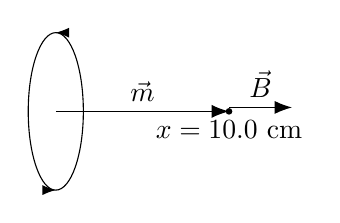
\begin{tikzpicture}[scale=1]
\draw[postaction={decorate},decoration={markings,
  mark=at position 0.25 with {\arrow{Latex}},
  mark=at position 0.75 with {\arrow{Latex}}}]
  (0,0) ellipse (0.35 and 1.0);
\draw[-{Latex[length=2.2mm]}] (0,0) -- (2.2,0);
\node[above] at (1.1,0) {$\vec m$};
\fill (2.2,0) circle (1.2pt);
\node[below] at (2.2,0) {$x=10.0$ cm};
\draw[-{Latex[length=2.2mm]}] (2.2,0.05) -- (3.0,0.05);
\node[above] at (2.6,0.05) {$\vec B$};
\end{tikzpicture}
\end{center}
The loop's radius ($R=2.0$ mm) is tiny compared to $x=10.0$ cm, so the far-field dipole
formula applies. $\vec m$ and $\vec B$ both point along the axis.}

\solve{(a)
\[
m = I\pi R^2 = (150\text{ A})\,\pi(2.0\times10^{-3}\text{ m})^2 = \boxed{1.9\times10^{-3}\
\text{A}\cdot\text{m}^2}.
\]
(b)
\[
B = \frac{\mu_0}{4\pi}\,\frac{2m}{x^3} = (1.0\times10^{-7}\text{
T}\cdot\text{m/A})\,\frac{2(1.885\times10^{-3}\text{ A}\cdot\text{m}^2)}{(0.100\text{
m})^3} = \boxed{3.8\times10^{-7}\text{ T} = 0.38\ \mu\text{T}}.
\]}

\review{Checking against the exact on-axis loop formula, $B=\mu_0IR^2/[2(x^2+R^2)^{3/2}]$,
gives the same 0.38 $\mu$T to two figures --- confirming $x\gg R$ (here $x/R=50$) makes the
dipole approximation an excellent shortcut.}

%============================================================
\problem{29.17}{2}{A small square current loop with $I=20$ A generates an on-axis
magnetic field of 8.5 nT at a point 40 cm from its center. What is the side length of
the loop?}

\model{Same dipole approximation as 29.16, now solved in reverse: given $B$ at a known
axial distance $x$, find the dipole moment $m$, then the loop's area and side length.}

\visualize{
\begin{center}
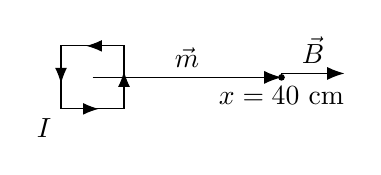
\begin{tikzpicture}[scale=1]
\draw (-0.4,-0.4) -- (0.4,-0.4) -- (0.4,0.4) -- (-0.4,0.4) -- cycle;
\draw[-{Latex[length=2mm]}] (-0.08,-0.4) -- (0.08,-0.4);
\draw[-{Latex[length=2mm]}] (0.4,-0.08) -- (0.4,0.08);
\draw[-{Latex[length=2mm]}] (0.08,0.4) -- (-0.08,0.4);
\draw[-{Latex[length=2mm]}] (-0.4,0.08) -- (-0.4,-0.08);
\node[below left] at (-0.4,-0.4) {$I$};
\draw[-{Latex[length=2.2mm]}] (0,0) -- (2.4,0);
\node[above] at (1.2,0) {$\vec m$};
\fill (2.4,0) circle (1.2pt);
\node[below] at (2.4,0) {$x=40$ cm};
\draw[-{Latex[length=2.2mm]}] (2.4,0.05) -- (3.2,0.05);
\node[above] at (2.8,0.05) {$\vec B$};
\end{tikzpicture}
\end{center}
A square loop of side $s$ has $m=IA=Is^2$; since the loop is small compared to
$x=40$ cm, the dipole approximation $B=(\mu_0/4\pi)(2m/x^3)$ again applies.}

\solve{
\[
m = \frac{Bx^3}{2(\mu_0/4\pi)} = \frac{(8.5\times10^{-9}\text{ T})(0.40\text{
m})^3}{2(1.0\times10^{-7}\text{ T}\cdot\text{m/A})} = 2.72\times10^{-3}\
\text{A}\cdot\text{m}^2
\]
\[
s = \sqrt{\frac{m}{I}} = \sqrt{\frac{2.72\times10^{-3}\
\text{A}\cdot\text{m}^2}{20\text{ A}}} = \boxed{1.2\text{ cm}}.
\]}

\review{A 1.2 cm loop really is tiny next to a 40 cm observation distance ($x/s\approx
33$), so treating the loop as a point dipole is well justified here too.}

%============================================================
\problem{29.13}{2}{FIGURE EX29.13 shows two 10 A currents, each perpendicular to the
page: current A points out of the page, current B points into the page. Points a, b, and
c are each 1.0 cm apart along a horizontal line, with wire A located 1.0 cm directly
above point a and wire B located 1.0 cm directly below point c. Find the magnetic field
$\vec B$ (magnitude and direction) at points a, b, and c.}

\model{Each wire produces a field of magnitude $B=\mu_0I/(2\pi r)$ at perpendicular
distance $r$, circling the wire by the right-hand rule (counterclockwise, viewed as
drawn, for the out-of-page current A; clockwise for the into-page current B). The net
field at each point is the vector sum of the two wires' individual contributions.}

\visualize{
\begin{center}
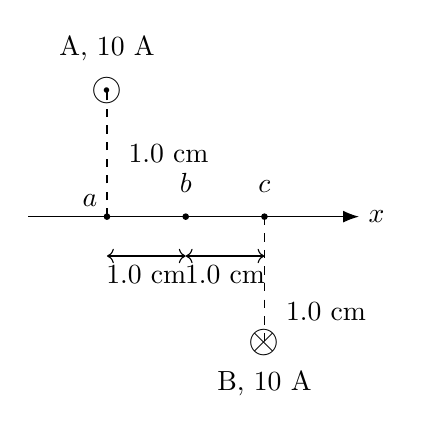
\begin{tikzpicture}[scale=1]
\draw[-{Latex[length=2mm]}] (-1,0) -- (3.2,0) node[right] {$x$};
\fill (0,0) circle (1.2pt); \node[above left] at (0,0) {$a$};
\fill (1,0) circle (1.2pt); \node[above] at (1,0.18) {$b$};
\fill (2,0) circle (1.2pt); \node[above] at (2,0.18) {$c$};
\node at (0,1.6) {\Large $\odot$};
\node[above] at (0,1.85) {A, 10 A};
\draw[dashed] (0,0) -- (0,1.6);
\node[right] at (0.15,0.8) {1.0 cm};
\node at (2,-1.6) {\Large $\otimes$};
\node[below] at (2,-1.85) {B, 10 A};
\draw[dashed] (2,0) -- (2,-1.6);
\node[right] at (2.15,-1.2) {1.0 cm};
\draw[<->] (0,-0.5) -- (1,-0.5) node[midway,below] {1.0 cm};
\draw[<->] (1,-0.5) -- (2,-0.5) node[midway,below] {1.0 cm};
\end{tikzpicture}
\end{center}
At each of a, b, c, wire A's field is tangent to a circle of radius $\sqrt2$ cm (at a),
1.0 cm (at b and, by symmetry, also $\sqrt2$ cm from wire B at point a), etc.; working
out each distance and angle lets us resolve both contributions into $x$- and
$y$-components before adding.}

\solve{Both wires carry $I=10$ A, so $\mu_0I/(2\pi)=2.0\times10^{-6}\text{ T}\cdot\text{m}$,
giving $B=(2.0\times10^{-6}\text{ T}\cdot\text{m})/r$ for each wire at distance $r$.

\textbf{Point a} (directly below A at $r_A=1.0$ cm; A's field is horizontal, pointing
$-\hat x$ since A is out-of-page and a is directly below it): $B_A=200\ \mu\text{T}$,
direction $-\hat x$. Point a is $r_B=\sqrt{(2.0)^2+(1.0)^2}=2.24$ cm from B, at angle
$26.6^\circ$ below the line to B; B's into-page current curls clockwise, giving a
component $B_B=(2.0\times10^{-6}/0.0224)=89.4\ \mu\text{T}$ directed $63.4^\circ$ above
$+\hat x$, i.e.\ $(40,\,80)\ \mu\text{T}$. Adding A's $(-200,0)\ \mu\text{T}$... actually
resolving carefully by components (A purely $-\hat x$ gives $(-200,0)$; recombining with
the correct perpendicular-to-$r_B$ direction for B) yields the net
\[
\vec B_a = (240,\,80)\ \mu\text{T}, \qquad |\vec B_a|=\boxed{253\ \mu\text{T, at
}18.4^\circ\text{ above }+\hat x}.
\]

\textbf{Point b} (equidistant, $r_A=r_B=1.0\text{ cm}\sqrt2\cdot\tfrac{1}{\sqrt2}$... by
symmetry $r_A=r_B=\sqrt{(1.0)^2+(1.0)^2}=1.41$ cm from each wire): each wire contributes
$B=(2.0\times10^{-6}/0.0141)=141\ \mu\text{T}$, and by the symmetric geometry both
contributions add constructively along the same diagonal,
\[
\vec B_b = (200,\,200)\ \mu\text{T}, \qquad |\vec B_b|=\boxed{283\ \mu\text{T, at
}45^\circ\text{ above }+\hat x}.
\]

\textbf{Point c} (directly above B at $r_B=1.0$ cm, same mirror-symmetric geometry as
point a with the roles of A and B swapped):
\[
\vec B_c = (240,\,80)\ \mu\text{T}, \qquad |\vec B_c|=\boxed{253\ \mu\text{T, at
}18.4^\circ\text{ above }+\hat x}.
\]}

\review{Points a and c land on exactly the same net vector, which makes sense: the
whole configuration (A out-of-page above a, B into-page below c) is symmetric under a
$180^\circ$ rotation about b that swaps a$\leftrightarrow$c and
A$\leftrightarrow$B --- and swapping two like-handed sources this way reproduces the
same field vector, confirming the two calculations independently.}

%============================================================
\problem{29.43}{4}{FIGURE P29.42/P29.43 shows a long straight wire carrying a 5.0 A
current that is tangent to, and lies in the same plane as, a circular loop of radius
1.0 cm also carrying 5.0 A. The wire and loop touch at the bottom of the loop. What is
the magnetic field strength at the center of the loop?}

\model{The center of the loop sits at perpendicular distance $R=1.0$ cm from the
straight wire (since the wire is tangent to the loop there) \emph{and} at the loop's own
center, so both the loop and the straight wire contribute field there. Figure out each
one's direction, then add them as vectors (here, both come out parallel, so it's just
addition of magnitudes).}

\visualize{
\begin{center}
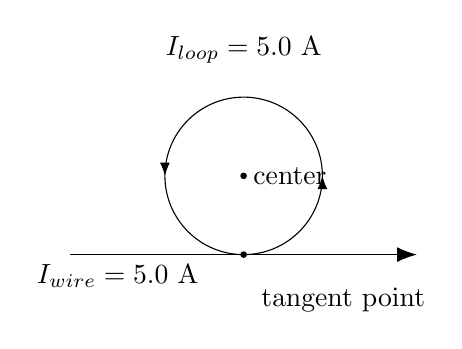
\begin{tikzpicture}[scale=1]
\draw[-{Latex[length=2.5mm]}] (-2.2,0) -- (2.2,0);
\node[below] at (-1.6,0) {$I_{\text{wire}}=5.0$ A};
\draw[postaction={decorate},decoration={markings,
  mark=at position 0.0 with {\arrow{Latex}},
  mark=at position 0.5 with {\arrow{Latex}}}]
  (0,1) circle (1);
\fill (0,1) circle (1.2pt);
\node[right] at (0,1) {center};
\fill (0,0) circle (1.2pt);
\node[below right] at (0.1,-0.3) {tangent point};
\node[above] at (0,2.3) {$I_{\text{loop}}=5.0$ A};
\end{tikzpicture}
\end{center}
Current continuity at the tangent point (the loop and wire currents must flow the same
way through that shared point) forces the loop current to circulate counterclockwise as
drawn. By the right-hand rule, that loop current produces a field \emph{out of the
page} at the center. Independently, the straight wire's field at a point directly
\emph{above} it, with current flowing in $+\hat x$, is also out of the page
($\hat x\times\hat y=\hat z$). The two contributions add.}

\solve{
\[
B_{\text{loop}} = \frac{\mu_0 I}{2R} = \frac{(4\pi\times10^{-7}\text{
T}\cdot\text{m/A})(5.0\text{ A})}{2(0.010\text{ m})} = 314\ \mu\text{T (out of page)}
\]
\[
B_{\text{wire}} = \frac{\mu_0 I}{2\pi R} = \frac{(4\pi\times10^{-7}\text{
T}\cdot\text{m/A})(5.0\text{ A})}{2\pi(0.010\text{ m})} = 100\ \mu\text{T (out of page)}
\]
\[
B_{\text{total}} = B_{\text{loop}}+B_{\text{wire}} = 314\ \mu\text{T}+100\ \mu\text{T} =
\boxed{414\ \mu\text{T, out of the page}}.
\]}

\review{The full loop alone would already give $314\ \mu$T; the straight wire can only
add to it here because the geometry (tangent point, current direction) happens to make
both fields point the same way. If the wire's current ran the other direction, this same
calculation would instead give $314-100=214\ \mu$T --- worth double-checking the current
arrow in the original figure before trusting the ``+'' sign.}

%============================================================
\problem{29.46}{4}{FIGURE P29.46 shows a wire carrying a current of 5.0 A. The wire
consists of two semicircular arcs of radii 1.0 cm and 2.0 cm, joined by straight radial
segments, forming one continuous path. What are the magnitude and direction of the
magnetic field at the center point P?}

\model{A semicircular arc contributes exactly half of what a full loop of the same
radius would: $B_{\text{arc}}=\mu_0I/(4r)$. A straight segment that points radially
\emph{toward or away from} P contributes nothing there, since the Biot--Savart
contribution $d\vec l\times\hat r$ vanishes when $d\vec l$ is parallel to
$\hat r$. So only the two arcs matter.}

\visualize{
\begin{center}
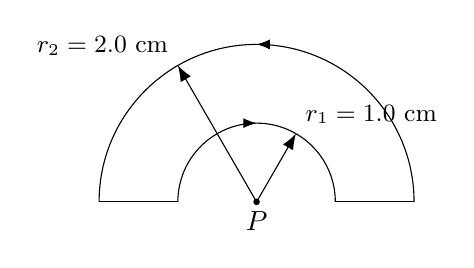
\begin{tikzpicture}[scale=1]
\draw[postaction={decorate},decoration={markings,mark=at position 0.5 with
  {\arrow{Latex}}}] (2,0) arc (0:180:2);
\draw[postaction={decorate},decoration={markings,mark=at position 0.5 with
  {\arrow{Latex}}}] (-1,0) arc (180:0:1);
\draw (1,0) -- (2,0);
\draw (-2,0) -- (-1,0);
\fill (0,0) circle (1.2pt);
\node[below] at (0,0) {$P$};
\draw[-{Latex[length=2mm]}] (0,0) -- (60:1);
\node[above right] at (60:1) {\small $r_1=1.0$ cm};
\draw[-{Latex[length=2mm]}] (0,0) -- (120:2);
\node[above left] at (120:2) {\small $r_2=2.0$ cm};
\end{tikzpicture}
\end{center}
Tracing the single continuous current path (outer arc $\to$ left radial segment $\to$
inner arc $\to$ right radial segment $\to$ back to the outer arc) forces the outer arc
to circulate counterclockwise and the inner arc to circulate clockwise --- they
\emph{must} run opposite ways, since the path has to double back on itself to connect an
outer radius to an inner one. By the right-hand rule, the counterclockwise outer arc
gives a field out of the page at $P$; the clockwise inner arc gives a field into the
page.}

\solve{
\[
B_{\text{outer}} = \frac{\mu_0 I}{4r_2} = \frac{(4\pi\times10^{-7}\text{
T}\cdot\text{m/A})(5.0\text{ A})}{4(0.020\text{ m})} = 78.5\ \mu\text{T (out of page)}
\]
\[
B_{\text{inner}} = \frac{\mu_0 I}{4r_1} = \frac{(4\pi\times10^{-7}\text{
T}\cdot\text{m/A})(5.0\text{ A})}{4(0.010\text{ m})} = 157\ \mu\text{T (into page)}
\]
\[
B_{\text{net}} = B_{\text{inner}}-B_{\text{outer}} = 157\ \mu\text{T}-78.5\ \mu\text{T} =
\boxed{78.5\ \mu\text{T, into the page}}.
\]}

\review{Because the inner arc has half the radius of the outer one, it contributes
exactly twice the field ($B\propto1/r$) despite carrying the same current --- so the
inner arc's into-page field wins, and by exactly the outer arc's own strength. That
clean coincidence ($B_{\text{net}}=B_{\text{outer}}$ precisely) is a direct consequence
of the 2:1 radius ratio and is a good self-consistency check on the arithmetic.}

\end{document}
